\documentclass{article}
\usepackage{tikz}
\usetikzlibrary{positioning}
\usetikzlibrary{decorations.markings}
\usepackage[dvipsnames]{xcolor}

\begin{document}

\title{Matrizen in Neuronalen Netzwerken}
\author{Tim Zollner}
\date{17.02.2025}
\maketitle

\section{Grafik}
    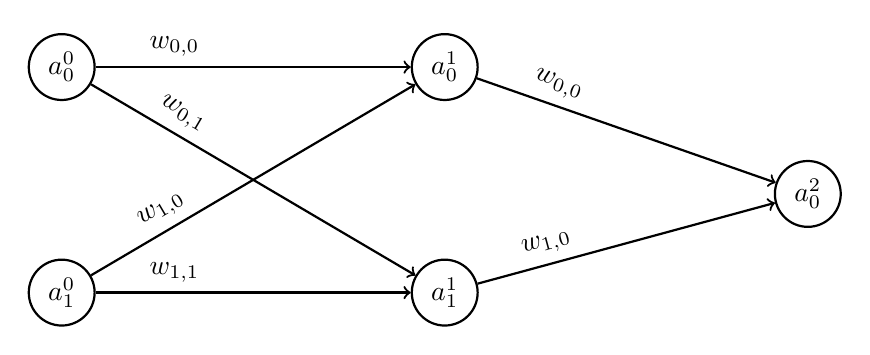
\begin{tikzpicture} [thick, main/.style = {draw, circle}]
        %Knoten
        \node[main] (00) {$a_0^0$};
        \node[main] (01) [below = 2cm of 00] {$a_1^0$};

        \node[main] (10) [right = 4cm of 00] {$a_0^1$};
        \node[main] (11) [right = 4cm of 01] {$a_1^1$};

        \node[main] (20) [below right = 1cm and 4cm of 10] {$a_0^2$};

        %Kanten
        \draw[->] (00) -- (10) node[pos=0.25, above] {$w_{0,0}$};
        \draw[->] (00) -- (11) node[pos=0.25, above, sloped] {$w_{0,1}$};
        \draw[->] (01) -- (10) node[pos=0.25, above, sloped] {$w_{1,0}$};
        \draw[->] (01) -- (11) node[pos=0.25, above] {$w_{1,1}$};
        \draw[->] (10) -- (20) node[pos=0.25, above, sloped] {$w_{0,0}$};
        \draw[->] (11) -- (20) node[pos=0.25, above, sloped] {$w_{1,0}$};



    \end{tikzpicture}

\section{Formeln}
    \[ a_0^1 = a_0^0 * \textcolor{OliveGreen}{w_{0,0}} + a_1^0 * \textcolor{OliveGreen}{w_{1,0}} + \textcolor{blue}{b^1} \]

\paragraph{}

allgemein:

\paragraph{}

\[  a_0^1 = \textcolor{blue}{b^1} + \sum_{k=0}^{n} a_k^0 * \textcolor{OliveGreen}{w_{k,0}}  \]




\end{document}